\section{Calculated Inputs}
\label{sec:usingStatisticalInput}
As described in the Section~\ref{sec:annSection} and in Figure~\ref{fig:overfitting} the Neural Network strives for a generalized function without over-fitting so that it also applies for data outside of the trained set. In order to achieve such a function it is necessary to include enough input parameters to get a close enough fit. Every input parameter should narrow down the possible number of output values and add more characteristics of the curve. What can become problematic is when the input parameters simply result in too many output values, e.g. if similar wind speeds, air densities and temperatures would correspond to wind productions between 800-1300 (see~\ref{sec:windPowerWindSpeed}). The generalization would move towards the majority of the wind productions in the interval but because the purpose of prediction is to come as close as possible to the ideal value this is not enough when the interval is too big. A possible solution is related to how the immediate behaviour of the price or production impacts what comes next --- volatility shown as many spikes indicates the underlying market condition\cite{yamin2004adaptive} and it could potentially help to generalize better if more characteristics of the spikes were to be included as input. It is apparent from Figures~\ref{fig:priceHourDevelopment400HoursStatistics} and~\ref{fig:windHourDevelopment400HoursStatistics} that price follows a certain trend and what comes next is highly influenced by the immediate previous hours. The prerequisite for adding it as input is the existence of a general recognizable pattern between the immediate past and the hours to predict but this must be investigated in the analysis and experiments. The approach will calculate the behaviour based on previous hours which also makes it applicable for 24-step-ahead forecasting since it can smooth out the transition when predicting by grounding in previous actual values. As discussed in Historical Data~\ref{sec:historicalData} the market has certain trends and if the prediction knows the production or price from one hour ago and the current market trend in general at a specific time, it will possibly have a better chance of guessing within a given interval. If putting this into context of the wind production interval 800-1300; the last hour wind production being 1100 and a rising current trend should with high probability not guess around 800 because the new input parameter is pulling in the other direction. The concept is illustrated in Figure~\ref{fig:WP}\todo{make drawing}. 

Problems can arise together with the inclusion of tendency --- when have we moved enough in one direction? We need to rely on the other input parameters to help pull us either up or down so that we can identify the next trend. The dataset used for training must be big enough to reflect coming trends or else problems can occur when meeting new trends in the unseen data for prediction, e.g. if most trends in general are rising in the training set and then trying to predict 24 hours that are not would result in a disproportion between the two sets. The possibility of over-shooting the first targets would be high since it has never seen such trends before. It will need to be tested thoroughly during our experiments. 

One thing to keep in mind here is that the trend and slope are only a minority of the input parameters. Without these the Artificial Neural Network would have made one generalization and the assumptions is that it will help the function to approach the target better when a lot of output possibilities exist. The result will be a new function where the immediate past is considered at every hour and the possibility of a improved generalization.

\begin{figure}[H]
\centering
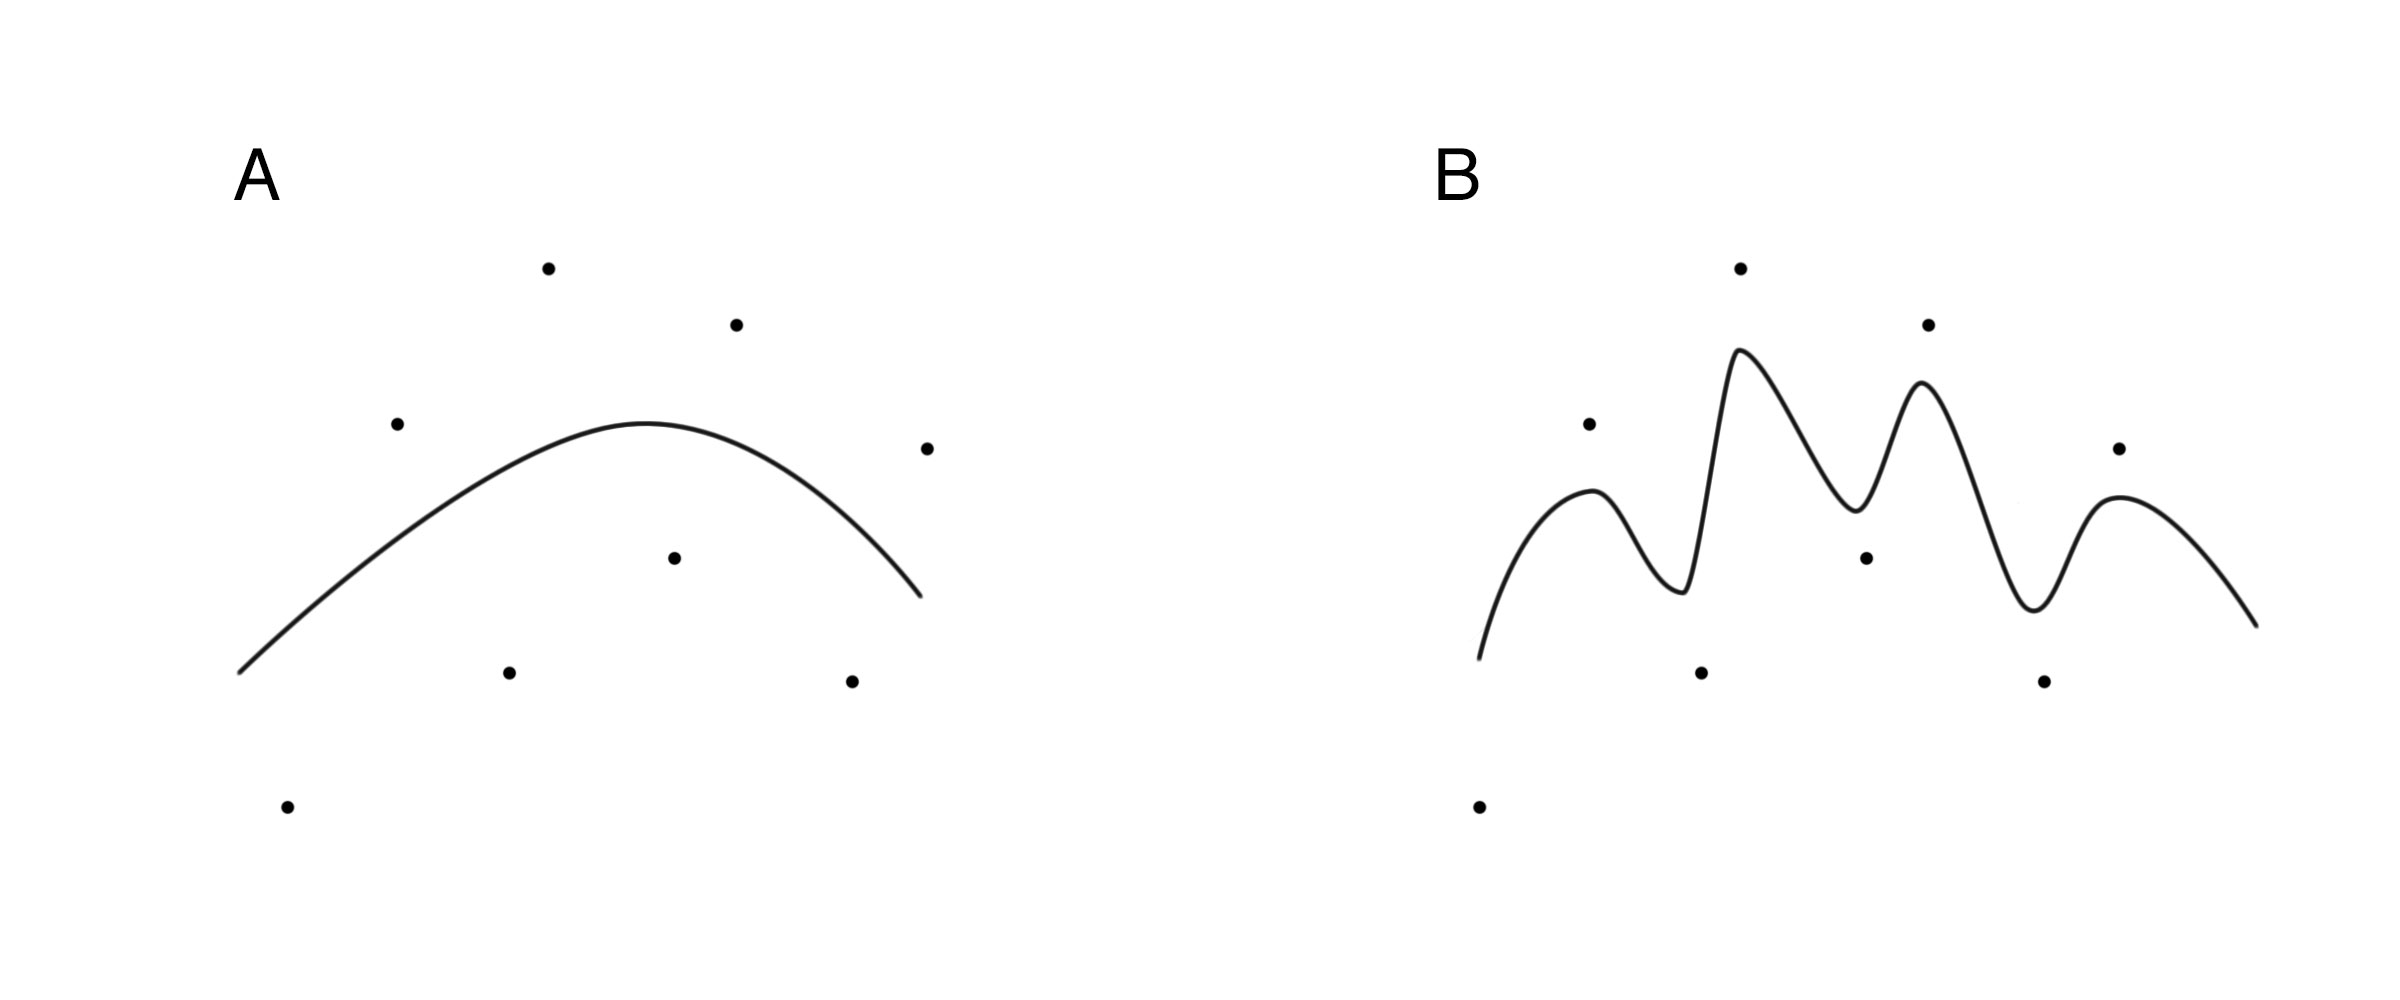
\includegraphics[width=0.99\linewidth,natwidth=898,natheight=587]{billeder/WP_000057.jpg}
\caption{A) Shows the generalized function. B) The approaching of output values}
\label{fig:WP}
\end{figure}

\begin{figure}[H]
\centering
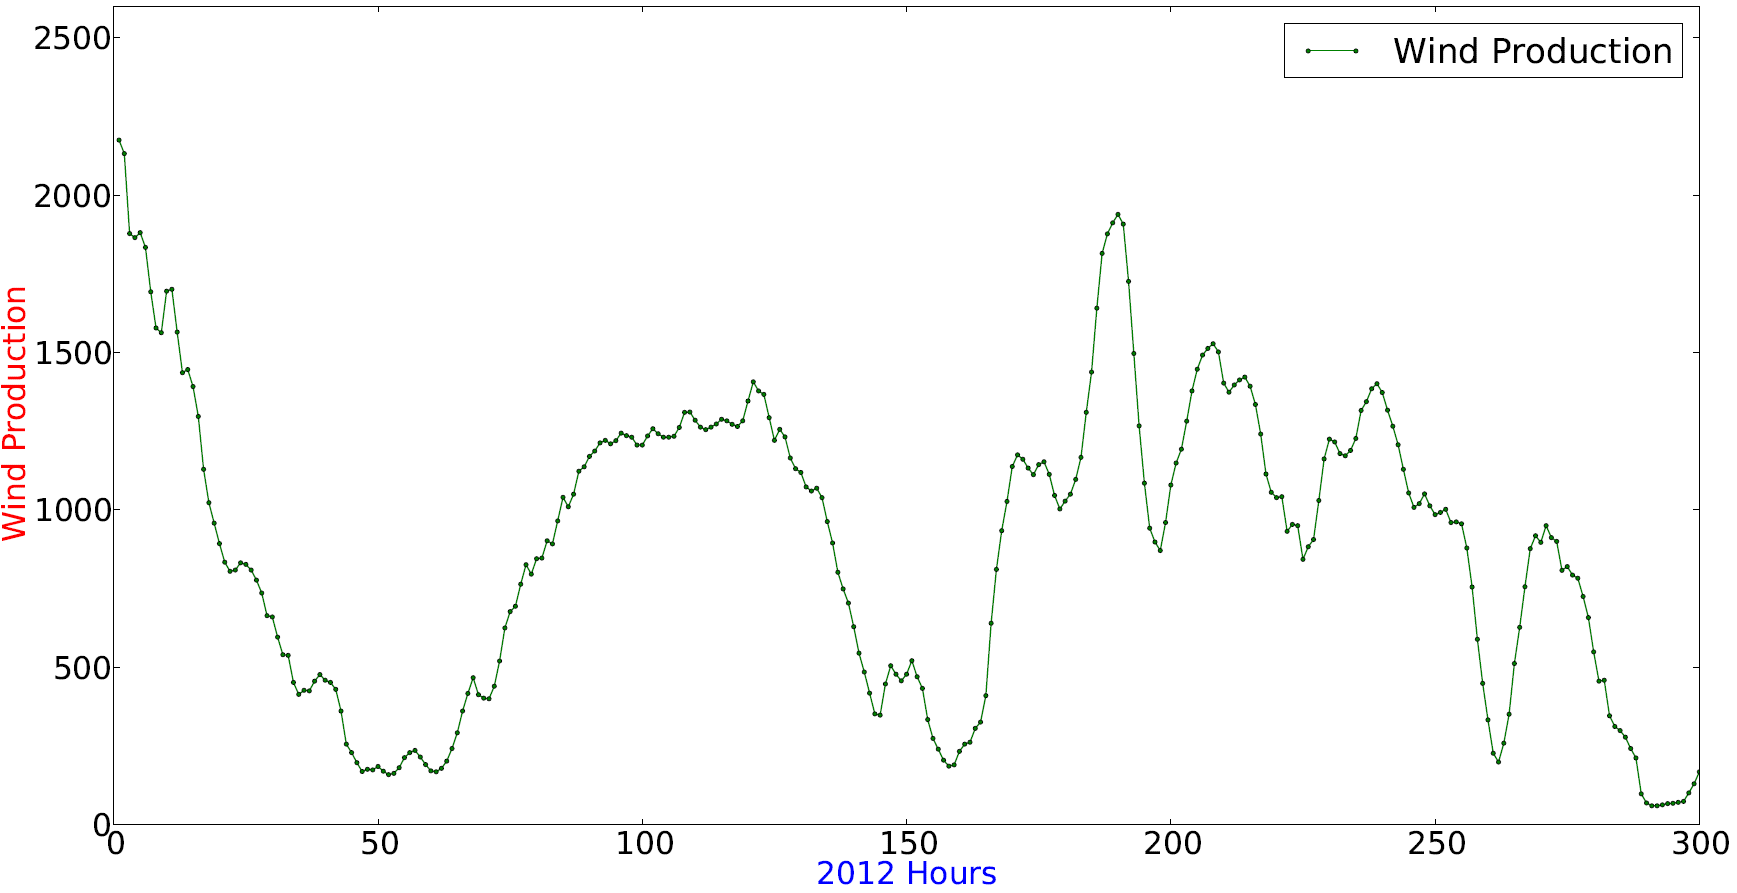
\includegraphics[width=0.99\linewidth,natwidth=898,natheight=587]{billeder/productionTendency400Hours.png}
\caption{Wind production development for 400 hours in 2011}
\label{fig:windHourDevelopment400HoursStatistics}
\end{figure}

\begin{figure}[H]
\centering
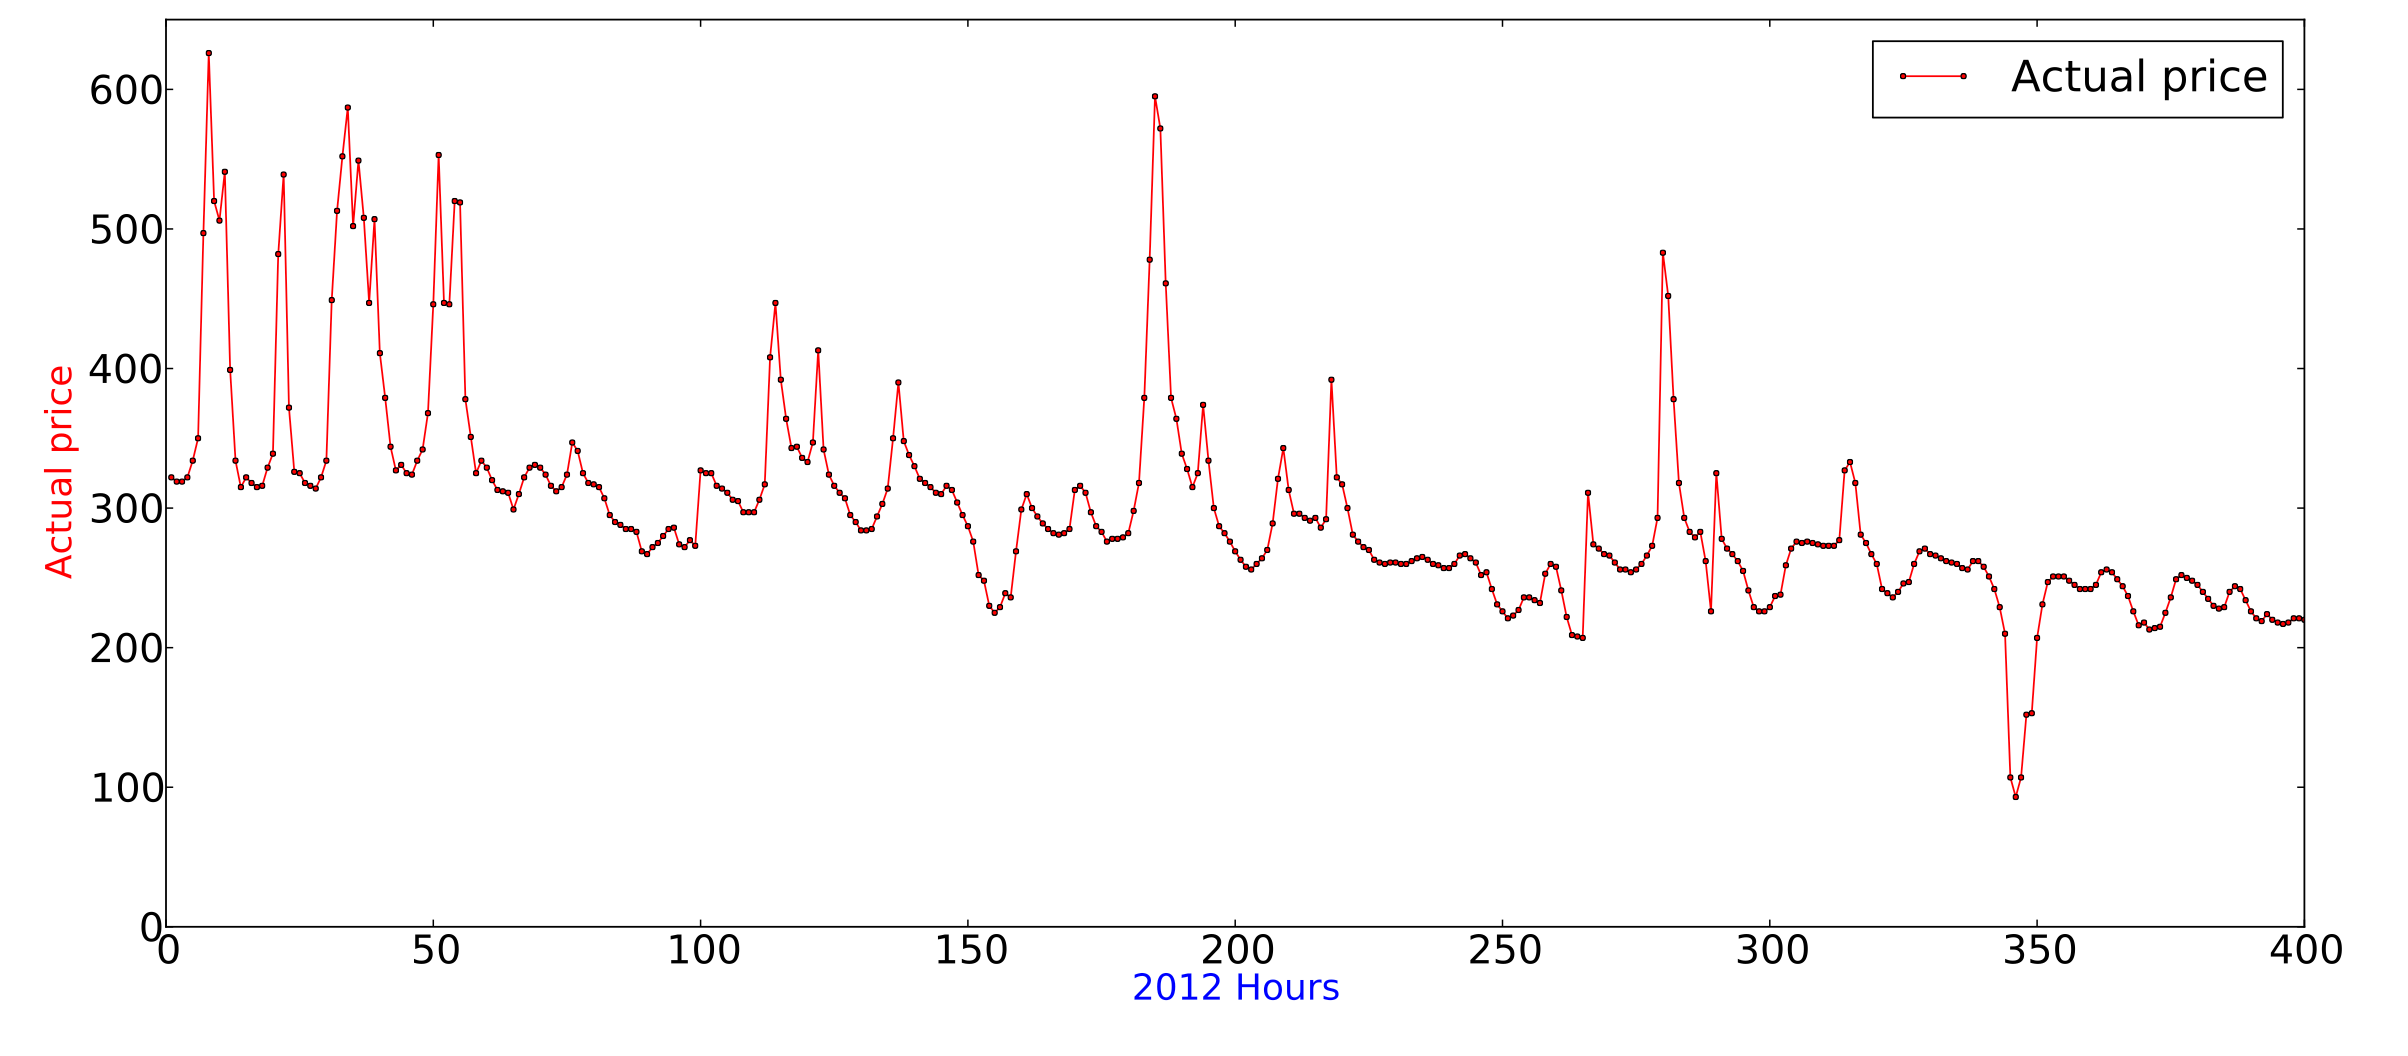
\includegraphics[width=0.99\linewidth,natwidth=898,natheight=587]{billeder/priceGraph400.png}
\caption{Price development for 400 hours in 2012}
\label{fig:priceHourDevelopment400HoursStatistics}
\end{figure}

We will experiment with different calculations that identifies something about current behaviour. The approaches will be used individually as well as together and will be described in the coming sections.

\subsection{Curve Analysis}
\label{sec:curveAnalysis}

\subsection{Scatter}
\label{sec:scatterStrategy}
Talk about how this can be a method to let the ANN itself calculate the impact of previous productions or prices and get the trend.

\subsection{EWMA - Historical Volatility}
\label{sec:ewmaVolatility}
\todo{Talk about statistical input features like historical volatility (EWMA), skewness and basic calculation of line slope. Skewness is a more sophisticated way of calculating if the distribution is leaning to one sine of the mean - the simple line slope calculation is meant to calculate if we are on the way up or down}

EWMA should be used for time series that do not have a clear trend direction\cite[Chapter~7.3.2]{econometrics} which is exactly what we have. \todo{see page 588 in econometrics book}. EWMA is a latent trend model where a latent variable is included to describe a discrete choice model. The latent variable is called the smoothing factor and if this factor is close to one then the last trend has a higher weight than the recent observation and when it is close to zero the new has higher priority and thereby letting the EWMA follow trends more rapidly - in our case the observation would be either production or price and the smoothing factor is calculated based on the last calculated trend. Choice of smoothing factor must be tested in experiments but since there is high volatility in both price and wind power production a lower factor could be expected. Every hour must calculate the historical volatility based on a defined number of previous hours. The exact number will also be found in experiments.

\subsection{Skewness}
\label{sec:skewness}



TEGNING MULTIPE STEP

TALK ABOUT MULTIPLE-STEP-AHEAD FORECASTING --> see karlbranting
